\documentclass{article}
\usepackage{tikz}
\usetikzlibrary{shapes.geometric}

\begin{document}

\begin{figure}[h]
    \centering
    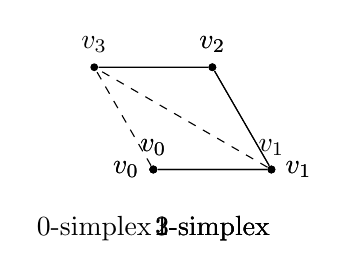
\begin{tikzpicture}[scale=1.5]

        % 0-simplex
        \node[circle,fill,inner sep=1pt,label={above:$v_0$}] (v0) at (0,0) {};
        \node[draw=none] at (-0.5,-0.5) {0-simplex};

        % 1-simplex
        \node[circle,fill,inner sep=1pt,label={above:$v_0$}] (v0) at (0,0) {};
        \node[circle,fill,inner sep=1pt,label={above:$v_1$}] (v1) at (1,0) {};
        \draw (v0) -- (v1);
        \node[draw=none] at (0.5,-0.5) {1-simplex};

        % 2-simplex
        \node[circle,fill,inner sep=1pt,label={left:$v_0$}] (v0) at (0,0) {};
        \node[circle,fill,inner sep=1pt,label={right:$v_1$}] (v1) at (1,0) {};
        \node[circle,fill,inner sep=1pt,label={above:$v_2$}] (v2) at (60:1) {};
        \draw (v0) -- (v1) -- (v2) -- cycle;
        \node[draw=none] at (0.5,-0.5) {2-simplex};

        % 3-simplex
        \node[circle,fill,inner sep=1pt,label={left:$v_0$}] (v0) at (0,0) {};
        \node[circle,fill,inner sep=1pt,label={right:$v_1$}] (v1) at (1,0) {};
        \node[circle,fill,inner sep=1pt,label={above:$v_2$}] (v2) at (60:1) {};
        \node[circle,fill,inner sep=1pt,label={above:$v_3$}] (v3) at (120:1) {};
        \draw (v0) -- (v1) -- (v2) -- (v3) -- cycle;
        \draw[dashed] (v0) -- (v3);
        \draw[dashed] (v1) -- (v3);
        \node[draw=none] at (0.5,-0.5) {3-simplex};

    \end{tikzpicture}
\end{figure}

\end{document}